\documentclass[a4paper,12pt]{article}
\usepackage[utf8]{inputenc}
\usepackage{graphicx}
\usepackage{fancyhdr}
\usepackage[pdftex=true, hyperindex=true, colorlinks=true, linkcolor=blue,
            citecolor=cyan]{hyperref}
\usepackage[francais]{babel}

\begin{document}

\begin{titlepage}

\addtolength{\oddsidemargin}{-0.15in}
\addtolength{\textwidth}{0.5in}
\addtolength{\topmargin}{-.375in}
\addtolength{\textheight}{0.75in}

\begin{center}

\begin{tabular*}{6in}{l@{\extracolsep{\fill}}r}{Vivien Alger}&{À
    l'attention de Florent Devin,}\\
    {Éric Hostalery}&{Yannick Le Nir,}\\
    {Cédric Salvador}&{et Rémi Vernay}\\
    {Mathieu Vacher}
\end{tabular*}
\vspace*{\fill}

\textsc{\LARGE Étude de la faisabilité
d'un cluster de smartphones Android}\\
\vspace*{\fill}

\today
\end{center}

\end{titlepage}

\tableofcontents
\newpage

% Defining page style for the rest of the document
\pagestyle{fancy}
\fancyhf{}
\fancyhead[L]{Introduction}
\fancyfoot[C]{Vivien Alger, Éric Hostalery, Cédric Salvador et Mathieu Vacher}
\fancyhead[R]{\thepage}
\renewcommand{\footrulewidth}{1pt}
\renewcommand{\headrulewidth}{1pt}
  
\section*{Introduction}
Dans le cadre de notre projet de fin d’études nous avons choisi de nous
attarder sur le comportement d’un cluster de smartphones. Plus précisément sur
la plateforme Android, vu que c’est actuellement la plus “ouverte”, accessible
et répandue.\\ En effet, nous avons constaté que les terminaux mobiles
deviennent de plus en plus puissants depuis quelques années, au point que l’on
peut désormais faire tourner des systèmes d’exploitation comme GNU/Linux
dessus. Partant de ce constat, nous avons alors décidé d’explorer les
spécificités du calcul réparti sur de telles machines, et de nous concentrer
sur les aspects inhérents à ces plateformes que sont la consommation de la
batterie et les déconnexions/pertes de réseau intempestives.\\ Ainsi nous avons
cherché à mettre en place une gestion dynamique de l’architecture de calcul
pour gé́rer la consommation de batterie et la tolé́rance aux pannes lié́es au
ré́seau mobile.\\ Pour illustrer cette problématique, nous avons tenté de porter
Akka sur la plateforme Android en le couplant avec le service google cloud
messaging pour faire communiquer les différent téléphones.

\newpage

\fancyhead[L]{\leftmark}

\section{Problématique}
Lors des premières recherches sur le thème d’un cluster de smartphones nous
avons très rapidement trouvé des articles sur un projet similaire: Hyrax. Ce
projet est une adaptation du framework Hadoop pour smartphones sous Android,
fait par des doctorants de l’université de Carnegie Melon aux États-Unis.\\ Ce
projet nous a beaucoup inspiré et nous a permis de tout de suite nous orienter
sur des pistes d’innovations en rapport avec notre thème. Ainsi l’un des
principaux défauts du projet Hyrax est qu’il ne prend pas en compte les
spécifités de la plateforme utilisée: les doctorants se sont “contentés” de
porter une partie d’Hadoop sur la machine virtuelle Dalvik d’Android. Les
problématiques liées à l’utilisation de téléphones tels que la gestion de la
batterie, des réseaux et autres furent donc laissés en tant que travaux futurs
à réaliser.\\ C’est de cet état de fait que nous sommes partis pour développer
notre problématique principale: mettre en place une gestion dynamique de
l’architecture de calcul pour gé́rer la consommation de batterie et la tolérance
aux pannes liées au réseau mobile. L’intérêt de cette problématique étant pour
nous de nous attarder autant que possible sur l’aspect mobile plutôt que la
partie calcul de l’architecture, qui a déjà été traitée largement par des
projets comme Hyrax.\\

\section{Pistes architecturales}

\subsection{Architecture type Hadoop}
Le premier type d’architecture vers laquelle nous aurions pu nous tourner est
celle d’Hadoop, reprise par exemple par le projet Hyrax. Dans ce cas, nous
avons un serveur, le namenode, qui va lancer les calculs et les distribuer sur
les différents noeuds du cluster.  Pour adapter ce type d’architecture au cas
mobile, on pourra penser au fonctionnement suivant : lorsqu’un téléphone veut
lancer un calcul, il va contacter le serveur avec le calcul désiré. Le serveur
va alors se charger de répartir les calculs sur les noeuds, récupérer le
résultat, et finit par le renvoyer au téléphone qui l’a demandé.

\begin{figure}[h]
\centering 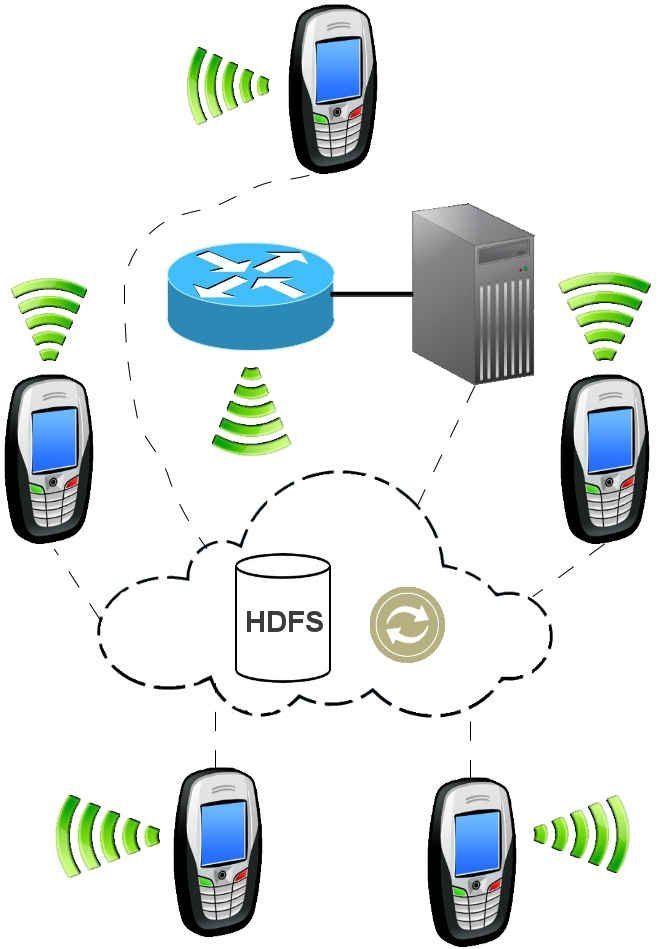
\includegraphics[scale=0.4]{images/hyrax.png}
\caption{Architecture du projet Hyrax}
\end{figure}

\newpage

\subsection{Architecture type Akka/Gridgain}
Le deuxième type d’architecture est du type Akka, utilisée par exemple par le
projet Akka-mobile : tous les acteurs sont indépendants, et chacun peut lancer
des calculs. Dans le cas d’un cloud mobile, nous devons quand meme utiliser un
serveur fixe dans le but de collecter les adresses ip des différents noeuds, et
de collecter des informations sur leur état. Néanmoins, contrairement au
premier cas, les calculs ne sont pas lancés depuis ce serveur, mais depuis un
téléphone qui sera utilisé comme client et qui utilisera les autres téléphones
disponibles comme workers pour le calcul.

\subsection{Architecture avec uniquement des SMS et base de données embarquée}
Une dernière piste d’architecture à laquelle nous avons pensé utiliserait des
SMS pour ses communications, et peut se découper en deux sous cas : avec ou
sans serveur fixe. Dans le premier cas, le serveur servirait seulement à
maintenir une base de données contenant tous les numeros de téléphone. Les
acteurs n’auraient alors plus qu’à récuperer ces numéros de téléphone et lancer
leurs calculs à leur convenance.\\ Dans le second cas, on indiquerait en “dur”
dans le code de l’application un numéro de téléphone qui serait en quelque
sorte la racine du cluster. Lorsque l’application est installée sur un nouveau
téléphone, ce dernier va envoyer un SMS à un téléphone racine afin de lui
signifier sa présence (ou son retrait dans le cas d’une désinstallation), et
celui ci fera alors un broadcast à tous les téléphones enregistrés jusqu’à
présent pour qu’ils aient la connaissance du nouveau.

\section{Application d'une architecture: tentative de portage d'Akka}
L’architecture que nous avons retenu est donc celle de type Akka. Même si les
trois étaient valables et nous auraient permis d’atteindre notre but, nous
avons voulu nous séparer le plus possible du serveur fixe, tout en gardant
l’option de différents modes de communications.\\ Pour mettre en place cette
architecture, le but était, dans un premier temps, de porter ce framework,
ainsi que Scala, sur Android, pour ensuite ajouter une surcouche
caractéristique aux plateformes mobiles. Cette surcouche se compose de l’ajout
de Google Cloud Messaging qui va permettre de connaître l’état, le status de la
batterie, et l’adresse ip des différents noeuds à tout moment, et de la partie
communication par SMS.

\newpage

\begin{figure}[h]
\centering
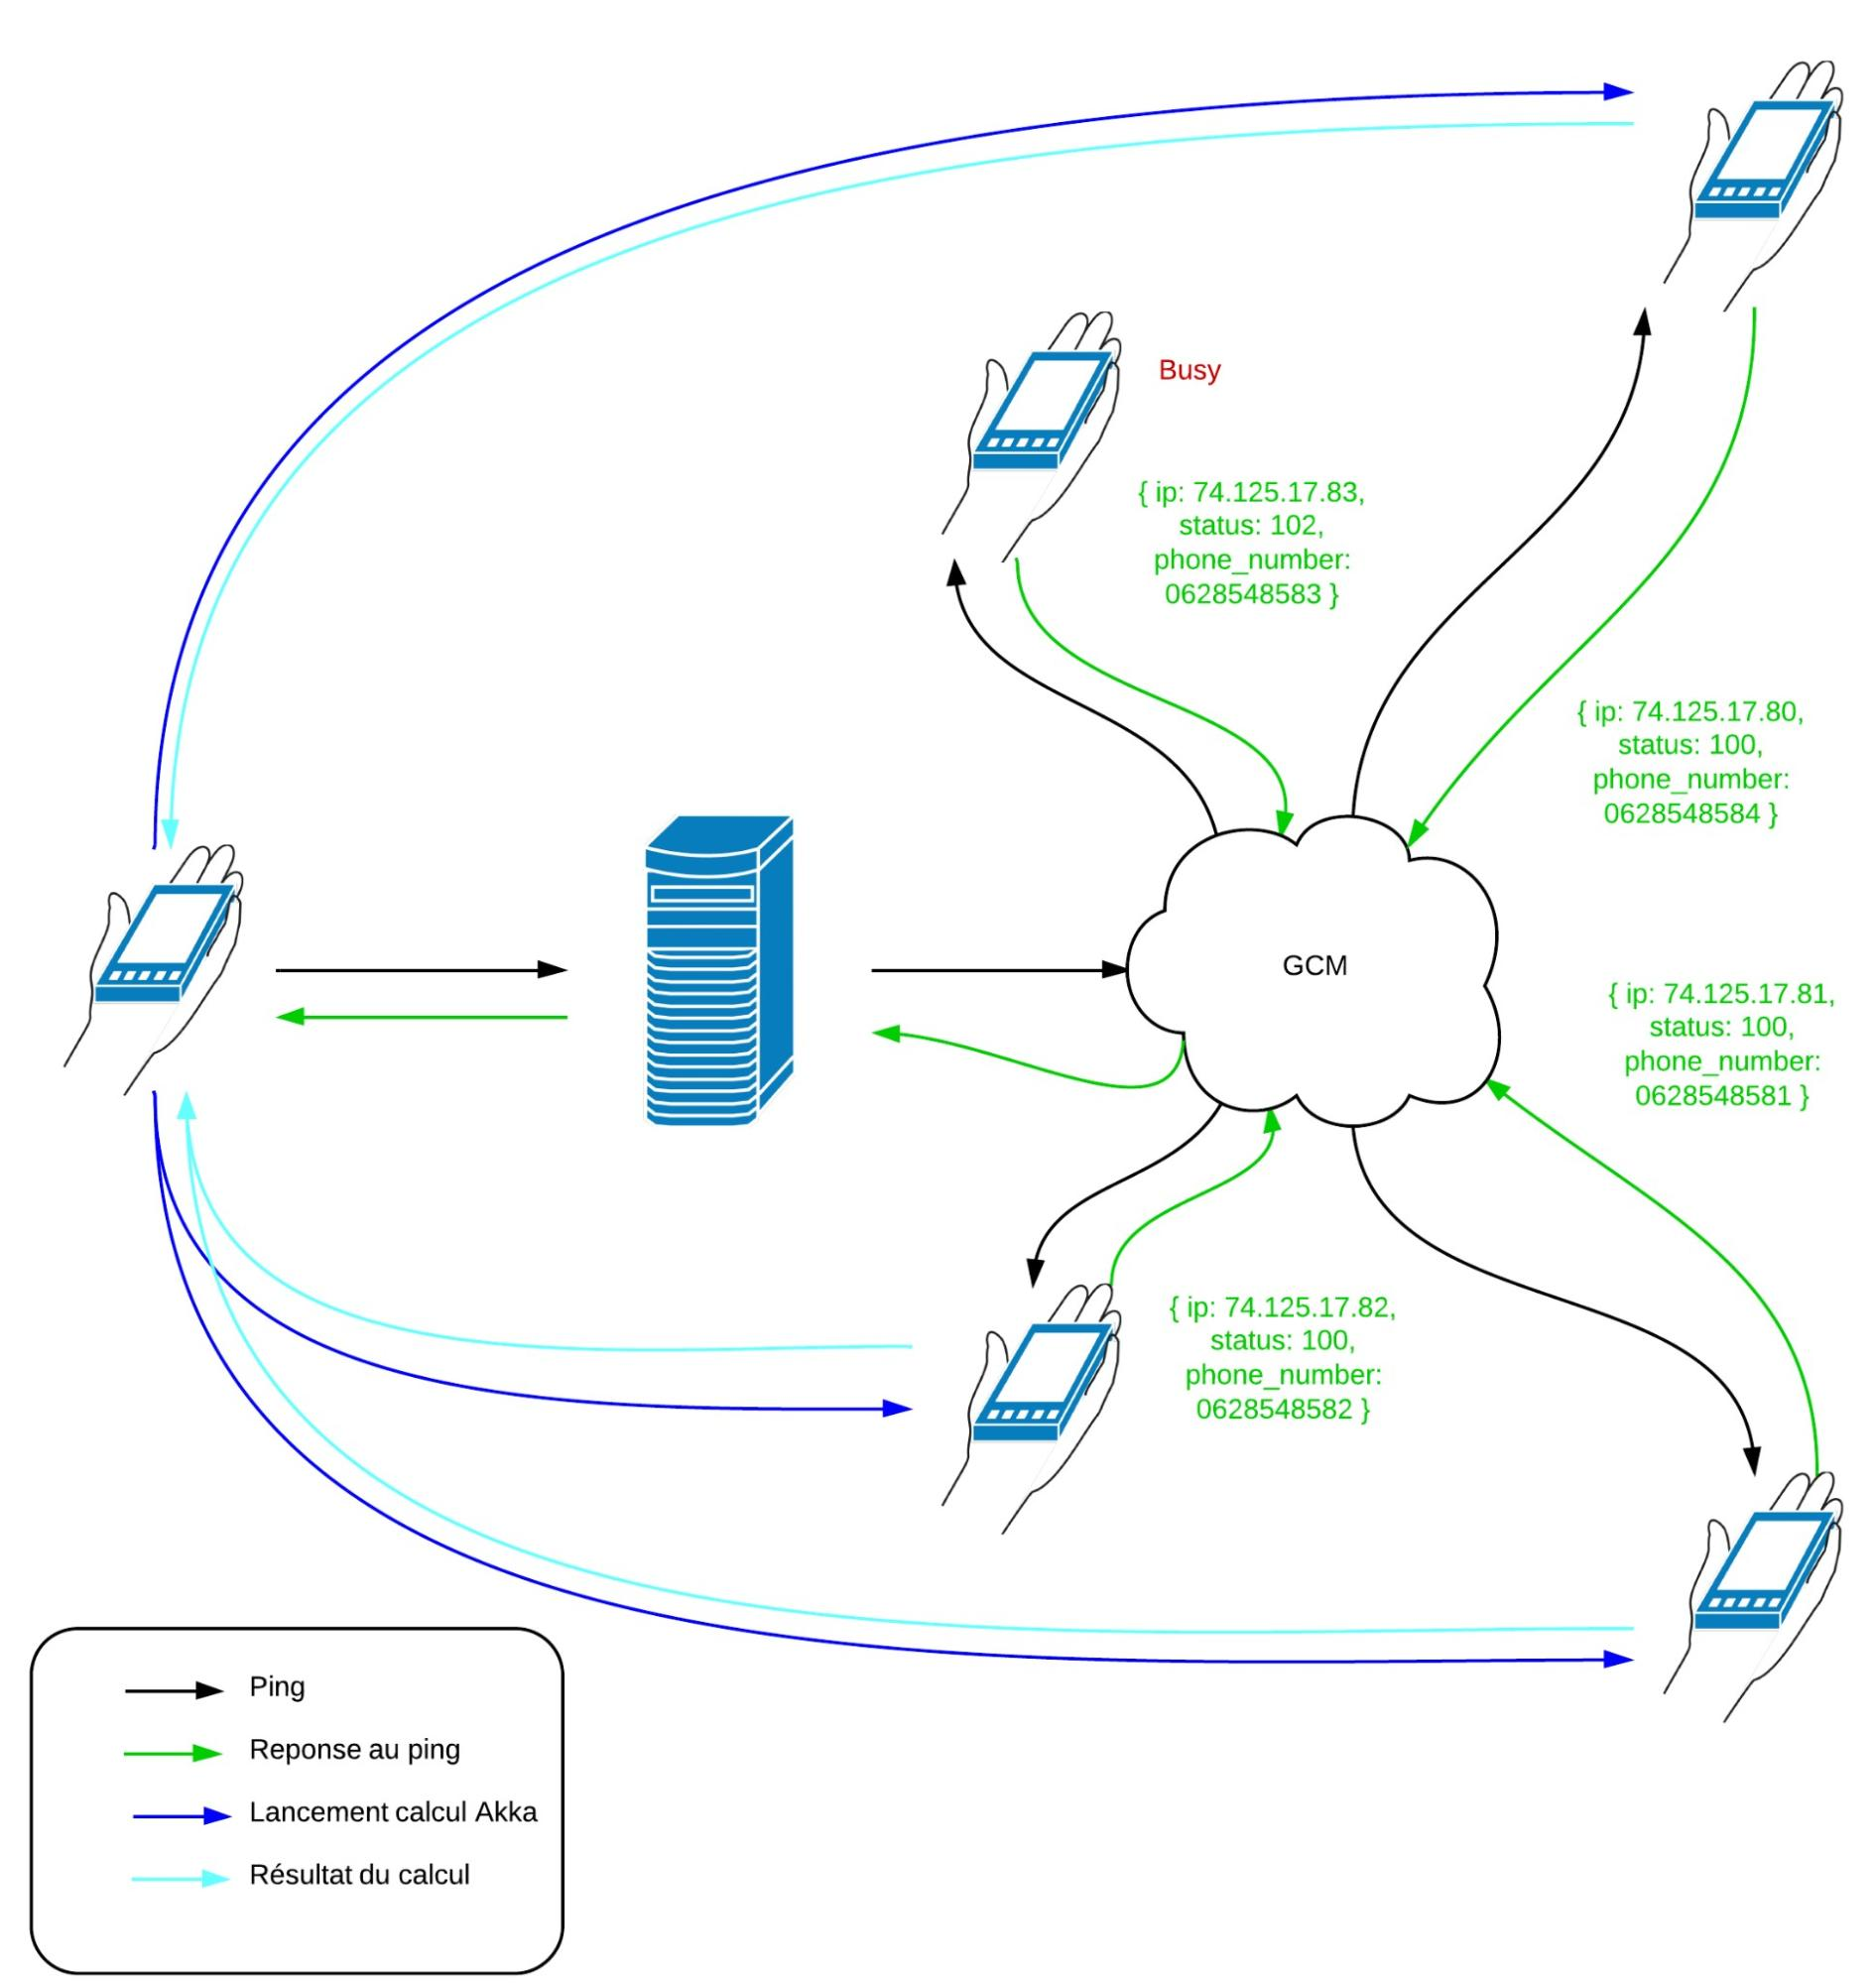
\includegraphics[scale=0.2]{images/gcm.png}
\caption{Schéma de notre architecture}
\end{figure}

\newpage

\subsection{Scala et Akka sur Android}

\subsubsection{Scala}
Nous avons décidé d'utiliser le langage Scala plutôt que le Java d'Android par
intérêt pour Scala, pour essayer quelque chose de nouveau et parce que son
paradigme fonctionnel est mieux adapté à la programmation concurrente
nécessaire pour la realisation du cluster. De plus, il est possible de
developper en Scala sur Android assez aisement, car c'est un langage qui tourne
déjà sur la JVM.\\ Scala nous parait plus attractif et intéressant pour le
développement Android que Java, et plus adapté que d’autres alternatives comme
Groovy ou JRuby car plus optimisé et moins gourmand en ressources.  Nous avons
commencé le développement avec Scala 2.9.2, la version déjà installée sur nos
machines et également celle proposée de base par le plugin SBT utilisé pour
initialiser la structure du projet, avant de finalement se tourner vers la
version 2.10.0 pour des raisons que nous évoquerons ultérieurement.\\


Nous avons été confrontés aux restrictions imposées par Android. La limite du
nombre de fonctions empêche d’utiliser les bibliothèques de Scala sans l’aide
d’un outil tiers tel que ProGuard. ProGuard nous a permis de compacter et
d’optimiser le code de notre application et des bibliothèques utilisées, malgré
une configuration parfois fastidieuse et des temps de compilation accrus, en
particulier si on ne désactive pas les options d’optimisation qui font exploser
la durée de compilation vers la quinzaine de minutes.

\subsubsection{Akka}
Pour faciliter la mise en place du cluster nous avons choisis d'utiliser en
plus de Scala, le framework Akka qui permettra de faciliter l'envoi de mes-
sages entre les différents noeuds du cluster. Le plus gros travail d'adaptation
se fera au niveau de ce framework, puisque dans le cas de l'utilisation de SMS
pour la communication il faudra intercepter le message, le reformater pour
l'envoyer par SMS, et lors de la reception le repasser à Akka
sous le bon format pour qu'il puisse travailler.\\


Nous avons eu beaucoup de mal à faire fonctionner les Remote Actors d’Akka.
Plusieurs problèmes se sont posés à nous:\\
\begin{itemize}
\item La configuration de Proguard est compliquée, à cause des dépendances de
  chacune des bibliothèques nécessaire. Proguard demande de fournir toutes ces
  dépendance, peu importe qu’on les utilise ou non. Il est possible de passer
  outre et de supprimer des warnings si on sait que l’on n’utilisera pas
  certaines fonctions ou bibliothèques, mais il faut le savoir au préalable. La
  configuration est donc un long et fastidieux travail de tâtonnement pour
  trouver le bon réglage. Cet outil a également posé des problèmes au niveau
  du traitement des modules de Akka. Tous ces modules conservent leur
  configuration par défaut dans des fichiers Reference.conf, que Proguard ne
  peut pas merger tout seul.\\
\item Nous avons également rencontrer des difficultés liées à nos versions de
  départ de Scala et Akka. Nous avons utilisé giter8 et sbt-android-plugin pour
  créer la structure initiale du projet, et avons gardé les versions de Scala
  et Akka proposées par défaut, soit Scala 2.9.2 et Akka 2.0.5. Plus tard, nous
  nous sommes aperçus que des incompatibilités entre Akka 2.0.X et Dalvik
  empêchaient les routeurs d’Akka de fonctionner. En effet, Akka 2.0.X faisait
  appel à des méthodes de la classe sun.misc.Unsafe, qui n’existe pas sur
  Dalvik, ce qui rendait l’application inutilisable. Pour régler ce problème,
  nous avons donc du passer à Akka 2.1 et donc Scala 2.10, et donc réécrire
  notre code pour tenir compte des évolutions de Scala et Akka. Entre autres la
  disparition de scala.concurrent.Ops et l’intégration de certaines features de
  Akka comme standard dans Scala.
\end{itemize}

\subsection{Utilisation de Google Cloud Messaging}

\subsubsection{Application mobile}
L’application mobile développée pour communiquer avec GCM reprend
l’architecture conseillée par google: elle comprend un broadcast receiver qui
va recevoir les messages envoyés par GCM, les passer à l’intent service qui va
gérer le message selon s’il s’agit d’un message d’enregistrement ou d’un
message de l’application.\\ Pour s’enregistrer avec GCM on utilise l’intent
com.google.android.c2dm
.intent.REGISTER (ou UNREGISTER pour le contraire), une
fois l’enregistrement réalisé, GCM renvoie l’identifiant du téléphone, qui est
ensuite envoyé au serveur tiers. Une fois l’enregistrement effectué, on peut
recevoir des messages transitant par GCM comme la demande de disponibilité(que
nous appelons couramment ping) qui va envoyer un message à tous les téléphones
enregistrés, qui à leur tour vont répondre en renvoyant leur disponibilité par
un status code proche du http, le numéro de téléphone enregistré dans
l’application et l’ip du téléphone.\\ Lors de la réalisation de cette
application, nous avons pu nous familiariser avec la gestion des appels réseaux
et des taches asynchrones sous Android. Cette gestion particulière nous à
causer quelques problèmes puisqu’il semble que les tâches asynchrones tournent
sur un seul et même fil d’exécution, or ceci vaut aussi pour l’intégralité des
appels réseaux, qui sont des tâches asynchrones. Ainsi nous ne pouvions pas
lancer une tâche appelant le serveur, puis avant de renvoyer la réponse à cette
tâche, envoyer un autre message au téléphone pour en obtenir les
informations. Pour contourner ce problème, nous avons enlever l’appel pour les
informations du téléphone qui demandait les informations sur le cluster.

\subsubsection{Serveur}
Pour toute application Google Cloud Messaging, il est nécessaire de créer un
serveur tiers servant d’intermédiaire entre les téléphones portables et les
serveurs de Google.  Ce serveur a été réalisé en Nodejs, car c’est un framework
efficace pour mettre à disposition des web services.  Du fait que nous devions
pouvoir accéder à ce serveur depuis nos téléphones portables, nous n’avons pas
pu utiliser un serveur fourni par l’école.\\
Ce serveur est couplé avec une base de données MongoDB, et met à disposition
plusieurs services :\\

\begin{itemize}
\item l’enregistrement d’un téléphone portable en base de donnée
  (registrationID et numéro de téléphone)\\
\item la mise à jour/suppression d’un téléphone portable\\
\item le lancement d’un ping à tous les téléphones portables enregistrés en
  base de données
\end{itemize}

Ce ping va nous servir à récupérer les adresses ip des téléphones portables,
ainsi que leur statut (disponible, occupé, ou batterie faible). Ces
informations doivent ensuite être transmises à Akka afin de créer le router et
de lancer les calculs, en laissant les téléphones communiquer directement entre
eux.\\


Néanmoins, comme nous l’avons évoqué dans la partie sur le portage
d’Akka sur Android, nous n’avons pas réussi à faire fonctionner les remote
actors sur cette plateforme jusqu’à très récemment, nous avons donc étudié
d’autres possibilités d’implémentation.  Une solution qui aurait donc pu être
viable, mais que nous n’avons pas eu le temps de tester et d’implémenter,
aurait été de faire passer toutes les communications par GCM. Nous n’aurions
donc plus eu besoin de connaître les adresses ip des acteurs, mais seulement
leur état. Une fois l’état du cluster connu, il aurait fallu redéfinir un
router (du type round robin par exemple), afin de répartir les calculs
efficacement entre les différents acteurs. Grâce à GCM toujours, nous aurions
pu connaitre l’état des noeuds à tout moment, et éventuellement récupérer plus
d’informations lors d’un ping, si nécessaire.

\subsection{Intégration avec des SMS}
La principale partie de notre projet que nous n’avons pas pu implémenter au
cours de notre projet est la communication par SMS.  Pour cette intégration,
plusieurs aspects sont à prendre en compte : la communication entre les acteurs
pour tout ce qui concerne Akka, et la communication avec le serveur GCM.\\

En ce qui concerne la communication des acteurs pour Akka, il aurait fallu
implémenter une sérialisation/desérialisation des messages transmis par Akka,
procédé qui aurait également pu être utilisé pour transmettre ces messages par
GCM.\\
Pour le deuxième aspect, plusieurs solutions auraient été envisag
eables :\\
\begin{itemize}
\item la première est d’utiliser un service externe, de type Twilio, qui a
  comme principal inconvénient d’engendrer des frais supplémentaires. Ce
  service permet d’envoyer et de recevoir des SMS depuis un serveur. En le
  couplant à notre serveur GCM existant, cela nous permettrait d’inclure a
  notre cluster des téléphone n’ayant aucun moyen de communiquer en data.\\
\item la deuxième solution serait d’utiliser un téléphone qui servirait de
  “pont” entre le cluster et le serveur GCM : il receptionnerait tous les SMS,
  et s’occuperait de tout transmettre au serveur en data.
\end{itemize}

Dans tous les cas, cela impliquerait d’ajouter à notre application Android la
gestion des SMS : si le SMS présente un certain format, alors notre application
va le prendre en charge et appeler abortBroadcast(); afin que tout soit
transparent pour l’utilisateur (pas de notification intempestive).

\subsection{Alternative avec le projet Akka-Mobile}
Nous avons trouvé assez tardivement un projet, nommé Akka-Mobile, très proche
de ce que nous voulions faire. L’auteur utilise le fonctionnement suivant :\\
\begin{itemize}
\item Le téléphone servant de client se connecte au serveur, obtient la
  référence d’un remote actor, par exemple l’actor “John” et lui envoie un
  message.\\
\item Le serveur associe une connexion TCP avec l’identifiant de l’appareil et
  transmet le message à l’actor ciblé\\
\item L’actor traite le message. Il peut ensuite renvoyer des messages, ou il
  peut aussi donner la référence de l’actor à d’autres qui vont s’occuper de
  répondre.\\
\item Quand un message doit être renvoyé sur un téléphone, le serveur vérifie
  que la connexion est toujours active.\\
\item …et envoie les réponses à l’actor qu’il faut sur le téléphone.\\
\end{itemize}
Quand il n’y a aucune connexion entre le serveur et le téléphone on utilise le
service C2MD(devenu GCM). Un message est envoyé à travers ce service pour dire
au téléphone que des réponses sont disponibles sur le serveur et qu’il doit se
connecter pour les obtenir.\\

Son code source étant disponible sur Github, nous avons pu le
regarder. Malheureusement, ce projet n’est plus maintenu depuis plus d’un an,
et n’est plus compatible avec les dernières versions d’Akka, Scala, et
Android. Nous avons essayé de le mettre à jour, mais nous nous sommes vite
rendus compte que le travail nécessaire était assez important, Scala et Akka
ayant bien évolués (ce qui est probablement la raison pour laquelle l’auteur ne
l’a pas maintenu).  Une autre possibilité aurait été de partir de zéro, et de
refaire de zéro la gestion du réseau en Scala. Le principal inconvénient de
cette solution est de perdre le travail fait sur Akka.

\newpage

\fancyhead[L]{Conclusion}

\section*{Conclusion}
Les possibilités de “cloud mobile” sont nombreuses et variées, et beaucoup de
travail reste à faire dans ce domaine. La meilleure solution serait
probablement de recréer un framework nativement destiné aux plateformes
mobiles, en reprenant les idées des acteurs majeurs du marché fixe, comme
Hadoop ou Akka. Repartir de zéro enlèverait ainsi les limitations et problèmes
de compatibilité auxquels nous avons du faire face lors du portage d’Akka sur
Android, comme les nouvelles dépendances apportées par les nouvelles versions,
qui rendent les projets de ce type peu maintenables.\\ De plus, nous pensons
que la partie SMS est un véritable atout par rapport aux clusters
traditionnels. En effet, cela nous permet de ne plus seulement nous reposer sur
un unique mode de communication, mais sur deux, ce qui permet de pallier des
pannes sur l’un des deux modes.\\ Néanmoins, il nous apparaît difficile de
faire un cluster composé uniquement de smartphones. En effet, durant les
calculs le client/maître à besoin de connaître les informations des différents
noeuds tels que leurs adresses IP ou leurs numéro de téléphone pour les SMS. Il
faut donc dans tous les cas une machine qui s’occupe de synchroniser les
changements de ces informations, rôle qui requiert d’être toujours disponible,
ce qui convient mal à un smartphone.\\ 

Pour revenir à notre problématique de base, si nous n’avons pas pu tester la
partie consommation de batterie par manque de temps et à cause de nos
problèmes, nous avons tout de même pu explorer la partie réseau avec nos
différentes architectures. On peut imaginer des utilisations pratiques si ce
projet était mené à bout.\\ Par exemple, il serait possible de créer un
équivalent ou un portage de BOINC(Berkeley Open Infrastructure for Network
Computing) pour smartphone, qui permettrait de prêter le temps de calcul
disponible de son téléphone à des projets scientifiques: pliage de molécules,
projet SETI...

\end{document}
